% Source: Wald GR, physical PDF p. 146
%         (printed p. 133).
% Coverage: Figure 6.1, equilibrium configurations of cold matter.
% Figures/tables/footnotes: Figure 6.1; no tables or footnotes.
% Status: source-reviewed and compile-clean.
% Uncertainties: none.
\begingroup
\renewcommand{\thefigure}{6.1}
\begin{figure}[htbp]
\centering
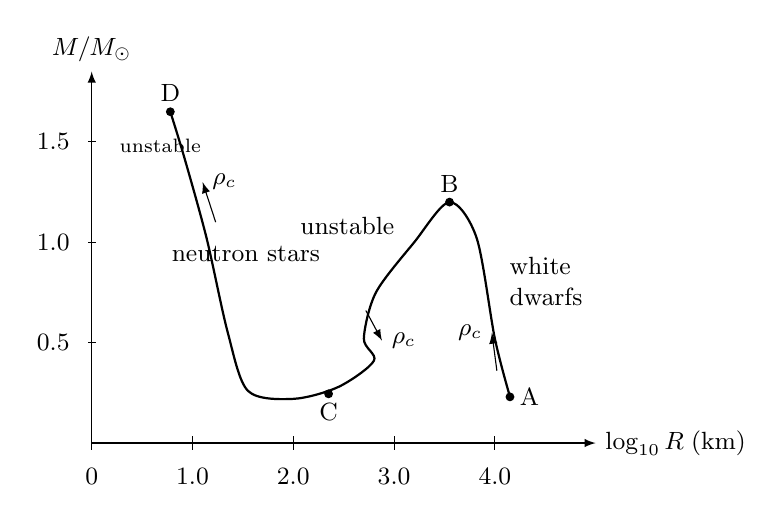
\begin{tikzpicture}[x=1.28cm,y=2.55cm,>=latex,font=\small]
  \draw[->] (0,0) -- (5.0,0) node[right] {\(\log_{10}R\;(\mathrm{km})\)};
  \draw[->] (0,0) -- (0,1.85) node[above] {\(M/M_\odot\)};
  \foreach \x/\lab in {0/0,1/1.0,2/2.0,3/3.0,4/4.0}
    \draw (\x,0.035) -- (\x,-0.035) node[below=3pt] {\lab};
  \foreach \y/\lab in {0.5/0.5,1/1.0,1.5/1.5}
    \draw (0.04,\y) -- (-0.04,\y) node[left=3pt] {\lab};
  \draw[thick,smooth] plot coordinates {
    (4.15,0.23) (4.00,0.52) (3.82,1.02) (3.55,1.20)
    (3.20,1.00) (2.82,0.75) (2.70,0.52) (2.80,0.41)
    (2.45,0.28) (2.00,0.22) (1.55,0.26) (1.35,0.55)
    (1.14,1.02) (0.92,1.42) (0.78,1.65)};
  \fill (4.15,0.23) circle (1.6pt) node[right] {A};
  \fill (3.55,1.20) circle (1.6pt) node[above] {B};
  \fill (2.35,0.245) circle (1.6pt) node[below] {C};
  \fill (0.78,1.65) circle (1.6pt) node[above] {D};
  \draw[->] (4.02,0.36) -- (3.97,0.55) node[left] {\(\rho_c\)};
  \draw[->] (2.72,0.66) -- (2.88,0.51) node[right] {\(\rho_c\)};
  \draw[->] (1.23,1.10) -- (1.10,1.30) node[right] {\(\rho_c\)};
  \node[anchor=west] at (4.05,0.88) {white};
  \node[anchor=west] at (4.05,0.73) {dwarfs};
  \node at (1.53,0.94) {neutron stars};
  \node[anchor=east] at (3.10,1.08) {unstable};
  \node[font=\scriptsize,anchor=west] at (0.18,1.48) {unstable};
\end{tikzpicture}
\caption{The equilibrium configurations of cold matter. Given an equation of state,
\(P=P(\rho)\), an equilibrium configuration is uniquely determined by the value
of the central density \(\rho_c\). The masses and radii of these configurations
are shown for values of \(\rho_c\) ranging from \(\sim10^5\,\mathrm{g\,cm^{-3}}\)
at point A to \(\sim10^{17}\,\mathrm{g\,cm^{-3}}\) beyond point D. In the white
dwarf regime, the values of \(M\) and \(R\) depend somewhat upon the assumed
composition of the star. In the neutron star regime, the values of \(M\) and \(R\)
depend greatly upon assumptions about the state of matter as well as assumptions
about the interactions between the fundamental constituents of matter. In this
latter regime, the figure is only a rough sketch of the qualitative features found
for most equations of state.}
\label{fig:6.1}
\end{figure}
\endgroup
